\subsection{Cross Talk}

Fig. \ref{fig:cross_talk1} shows the signal wave form of stopped channel and the front channel of typical proton event.
The signal wave form of stopped channel is differencial form of the that of the front channel.
Such signals are appeared at channel number 1 which cannot enter drifted ionization electron in electric power lines.
One possibility which cause such a phenomenon is following process.
The distance between anode channels is very short,
so the influence of mutual capacitance become large
and this capacitive coupling induce cross talk noise.
This effect notably appears the channel where the difference of the charge between adjacent channels is large,
such as the channel around stopped point of proton.
Then, we implement this phenomenon in Monte Carlo Simulation
by adding bipolar shape of the signals at adjacent channels.
The area of the mountain of bipolar shape is 10.5\% of the area of signal gaussian at each adjacent channel.
The value of 10.5\% is determined by comparing the hit charge distribuntion at stopped channel between data and MC simulation.
Fig. \ref{fig:cross_talk2} shows hit charge distribution of stopped channel.
Black is data and blue is MC simulation with cross talk and red is MC simulation without cross talk.
As shown in Fig. \ref{fig:cross_talk2}, data and MC simulation with cross talk is good agreement,
so the value of 10.5\% is reasonable.

\begin{figure}[htbp]
  \begin{tabular}{cc}
    \begin{minipage}{0.5\hsize}
      \centering
      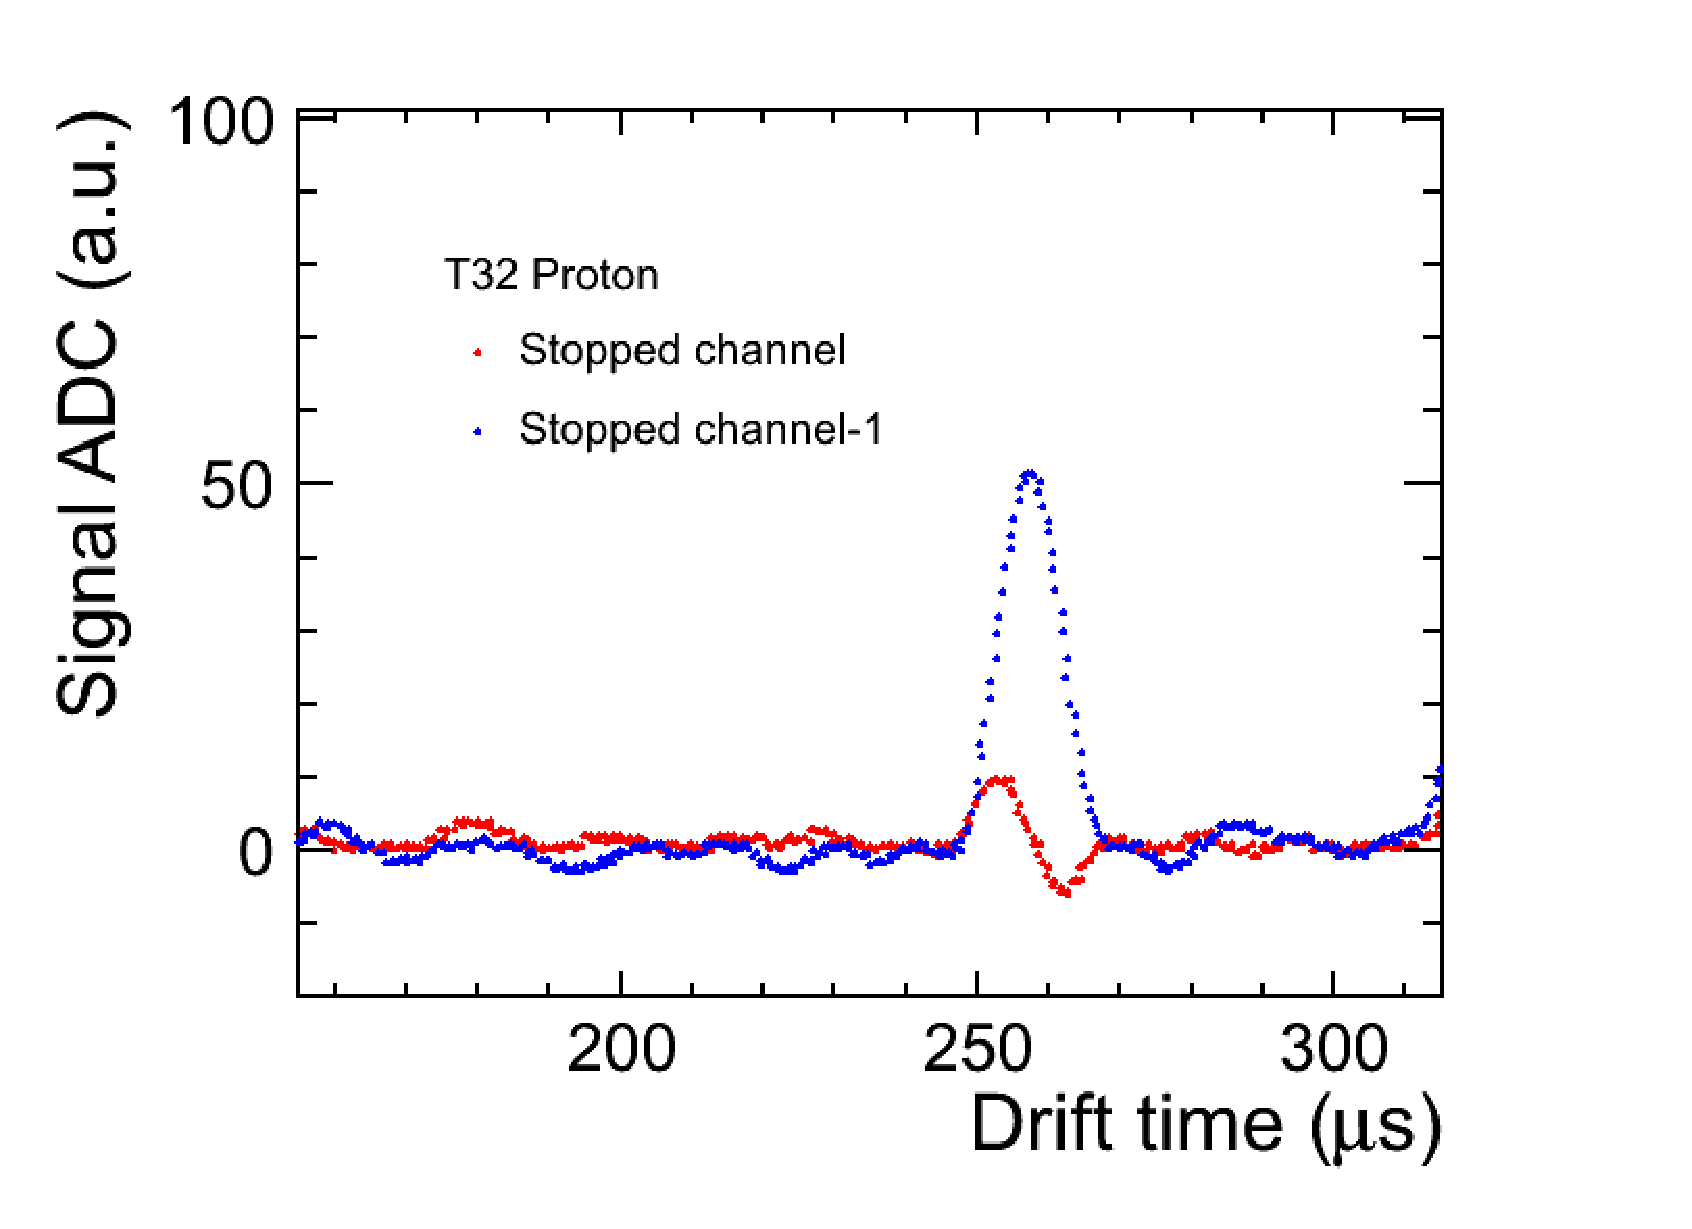
\includegraphics[width=6cm,clip]{fig/cross_talk_1.eps}
      \caption{Signal wave form of stopped channel and the front channel}
      \label{fig:cross_talk1}
    \end{minipage}
    \begin{minipage}{0.5\hsize}
      \centering
      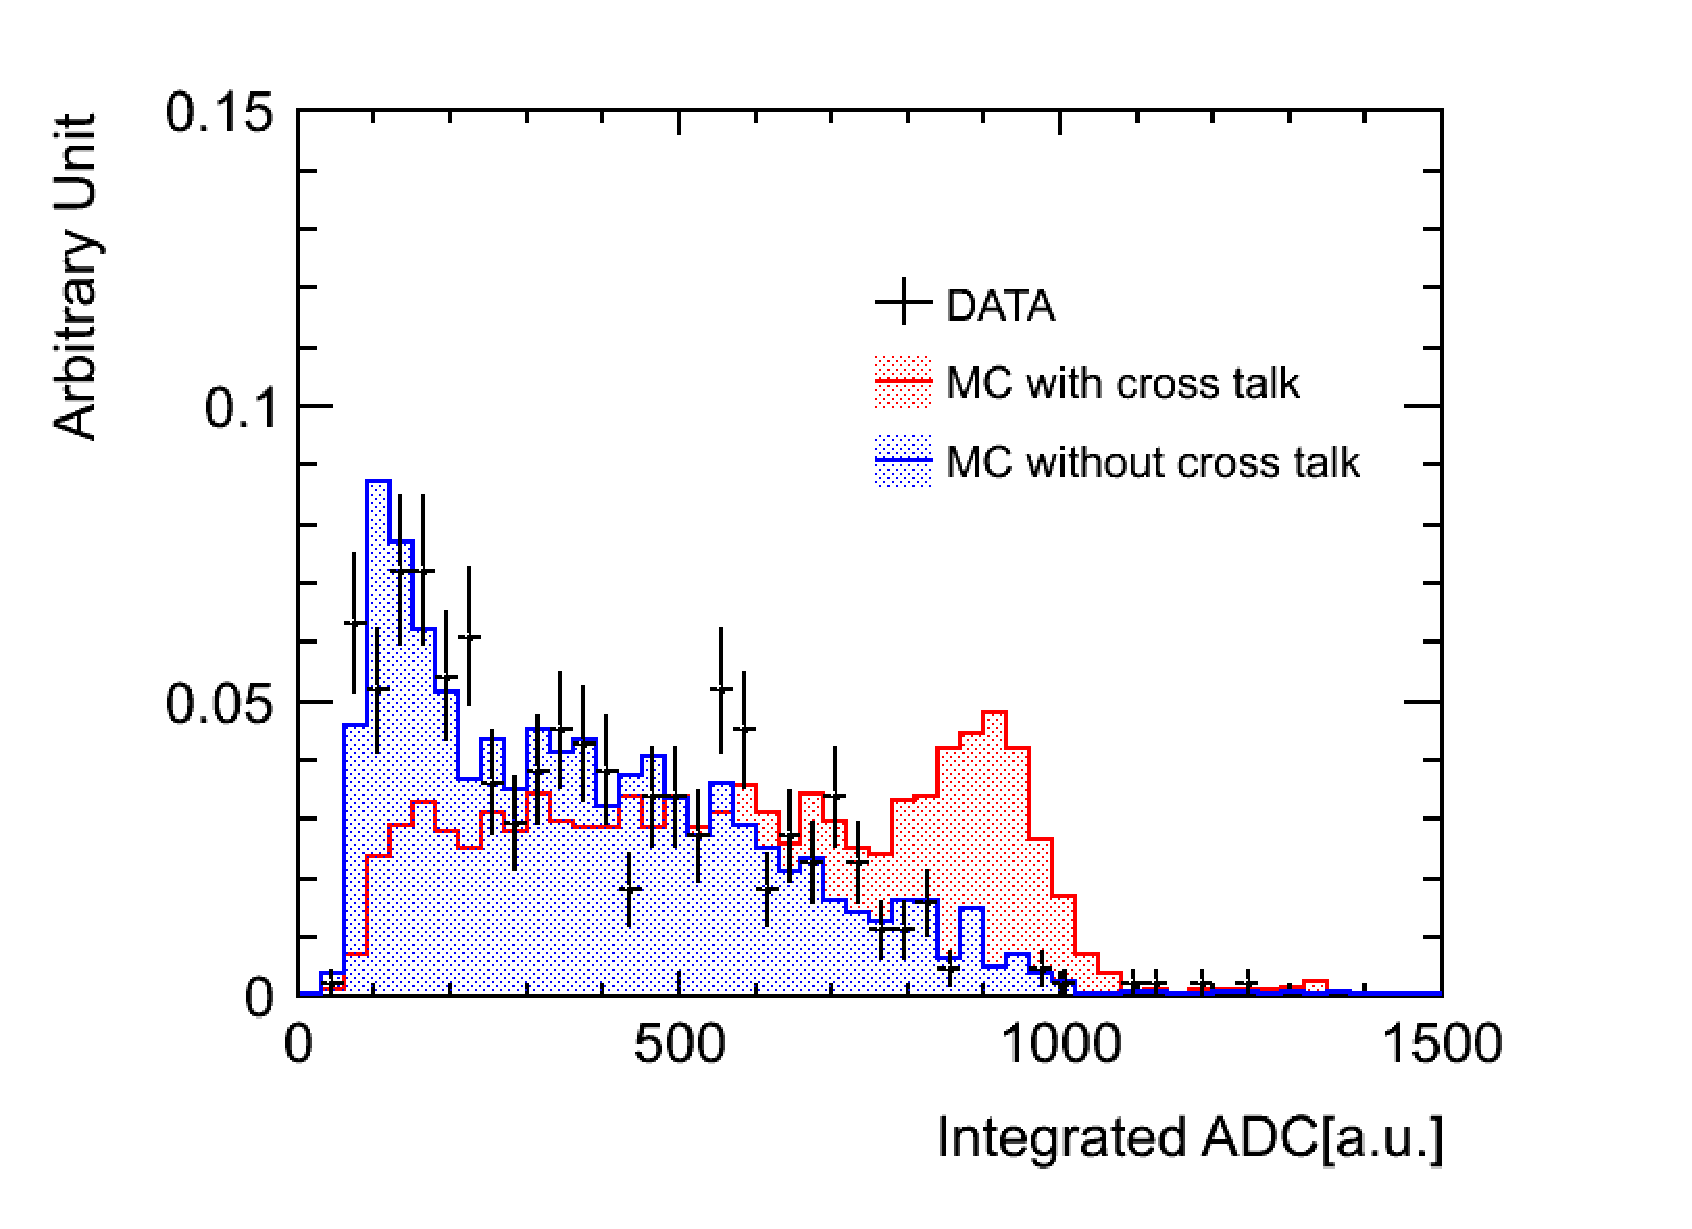
\includegraphics[width=6cm,clip]{fig/cross_talk_2.eps}
      \caption{Hit charge distribution of stopped channel}
      \label{fig:cross_talk2}
    \end{minipage}
  \end{tabular}
\end{figure}

% LocalWords:  differencial
